\newpage
\section{EEPROM memory}
The PSoC that is used in the Rolling Road has a little local EEPROM, what is used to save PID, wanted torque and offset values to the sensors.

\begin{figure}[H]
	\centering
	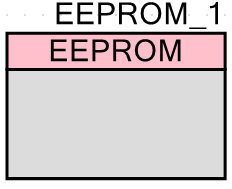
\includegraphics [width=1in]{Software/Pictures/EEPROM_block.PNG}
	\caption{PSoC top design EPPROM block}
	\label{fig:EEPROM_block}
\end{figure}

To the project there are build a class to make it more easy for the user to save data too the EEPROM. It is the same class that are used in the Motor controller for AU2. The class will automatic control where too write and read data from the EEPROM, and have little mechanism to check if there are data or not, so that some kind of guarantee that it not just reading some old fragmented information, that may make PID regulator unstable or give some funny readings. One off the down sites with this class: it work static. You have to tell the class have much data you want to save or read from it, in the initializing process of the class. Too see have to use the class goto page \pageref{table:Class_description_EEPROM_RR_PSoC}. \\
To use the EEPROM in the class, two function are used.

\lstset{language=C}
\begin{lstlisting}
#define START_EEPROM_SECTOR  (1u)
#define START_BYTE         ((START_EEPROM_SECTOR * EEPROM_SIZEOF_SECTOR) + 0x00)

cystatus EEPROM_1_WriteByte((uint8)data, START_BYTE + pos);
uint8 EEPROM_1_ReadByte(START_BYTE + pos);
\end{lstlisting}

The first function (line 1) are used to write new data to the EEPROM, it will write one byte, and return state of it has succeeded or not. The next function (lint 2) are used to get a byte from specific place. START\_BYTE are the start address of the EEPROM. 